
\chapter{\label{introduction}Introduction}

\section{Motivation}

The increasing number and diversity of networking devices is challenging the network research community. More and more applications and protocols are developed to address the needs of different platforms and use cases. For performance reasons, these protocols and applications are often tightly bound to each other. The resulting systems may then perform well, but lack of flexibility in the underlying architecture. This inflexibility is well demonstrated by the long lasting and still ongoing switch from IPv4 to IPv6 in the TCP/IP protocol stack of the current Internet architecture.

The Autonomic Network Architecture~(ANA)~\cite{ana} targets this problem with a fundamental change of paradigms. In ANA, all functionality is encapsulated in so called functional blocks. The size of functional blocks is a priori not defined. It may range from a minimalistic checksum calculation up to a huge holistic protocol stack. ANA provides a set of abstraction models and generic communication methods that the functional blocks use to interact with each other. This framework allows a completely isolated development of the algorithms running in the functional blocks. The operating system then interconnects the functional blocks and builds up an individual protocol stack. The device chooses the functional blocks for this protocol stack depending on the capabilities of the platform and the requirements of the running applications. The result is a flexible and dynamic protocol stack, that is able to adapt itself to any given situation and may change at runtime. Figure~\ref{protocolStack.eps} shows such a dynamic protocol stack and compares it to the inflexible, static and strongly layered protocol stack of the current Internet.

\begin{figure}
  \begin{center}
		 \includegraphics[scale=1.3]{protocolStack.eps}
  \caption{a) The strongly layered static protocol stack of the current Internet, b) The dynamically adaptable protocol stack of an ANA node}
  \label{protocolStack.eps}
  \end{center}
\end{figure}
The existing implementations of ANA \cite{ana}, \cite{lana} do not yet reach the performance of the traditional Internet architecture. This is due to two reasons. First of all, the level of indirection introduced by ANA trades some performance optimization features of the application for a higher flexibility and modularity of the overall system. The second reason is that the traditional Internet architecture benefits from a wide range of hardware support in the networking interface cards, which is not yet available for ANA. In order to compensate the performance penalty of ANA, a hardware acceleration for ANA is needed. It is not feasible to use application specific integrated circuits~(ASIC) for this purpose, since the functionality of these devices must be completely specified at design time. This static characteristic of ASICs would conflict with ANA's effort towards flexibility and adaptability.

The evolving partial reconfiguration capabilities of modern field programmable gate arrays (FPGA) combine the flexibility of a software implementation with the high-performance acceleration features of ASICs. L\"{u}bbers et. al.~\cite{towardsAdaptiveNetworkingForEmbeddedDevices} and Keller et. al.~\cite{reconfigurableNodesForFutureNetworks} therefore came up with the idea of porting ANA to a reconfigurable system on chip (rSoC). On these devices, a microprocessor core (either soft- or hardcore)  is combined with a programmable logic fabric. The software running in the microprocessor may then decide to offload the execution of computational intensive and frequently used functional blocks from the microprocessor to the programmable logic. Based on the partial reconfiguration features, this mapping of functional blocks to hardware or software can be adapted at runtime.

In order to reduce the engineering effort, L\"{u}bbers et. al.~\cite{towardsAdaptiveNetworkingForEmbeddedDevices} and Keller et. al.~\cite{reconfigurableNodesForFutureNetworks} further suggest to use ReconOS~\cite{reconos} as base system. In ReconOS, partially reconfigurable logic slots are used as so called hardware threads. These hardware threads appear to the software like normal software POSIX-threads. ReconOS enables the hardware threads to access operating system objects like semaphores, message boxes and shared memory. The combination of these mechanisms simplifiess the interaction of software and hardware elements. The suggested approach benefits from the hardware acceleration provided by ReconOS by implementing some functional blocks as hardware threads. Figure~\ref{reconosForAna.eps} shows the architecture of ReconOS and how the functional blocks are mapped to the hardware threads.

\begin{figure}
  \begin{center}
		 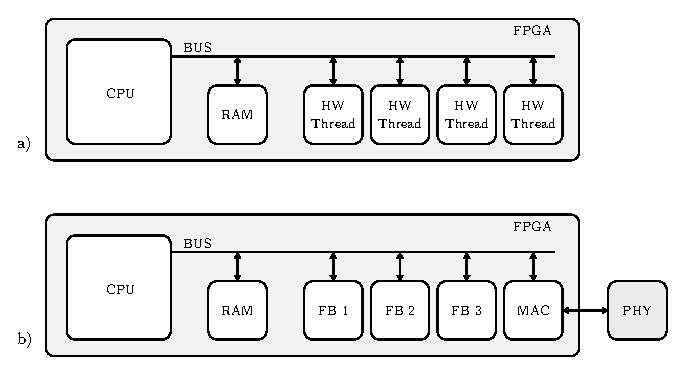
\includegraphics[width=\textwidth]{reconosForANA.eps}
  \caption{a) The ReconOS architecture: partially reconfigurable logic slots are used as hardware threads. b) Using ReconOS for ANA: a set of functional blocks is executed in hardware threads.}
  \label{reconosForAna.eps}
  \end{center}
\end{figure}
However, the major problem of this approach is the shared bus architecture of ReconOS. Especially with a data intensive application like ANA, the shared bus soon becomes the bottleneck of the system. 

\section{Aims of this Thesis}
In this thesis we present an extension of the ReconOS framework with a high-throughput communication infrastructure shown in figure~\ref{interconnectionInfrastructure.eps}. This infrastructure contains a packet based network on chip (NoC) that guarantees each hardware thread a worst-case incoming and outgoing data throughput. Additionally, a ring buffer based gateway is designed and implemented to speed up the transfer from software to hardware and vice versa.

\begin{figure}
  \begin{center}
		 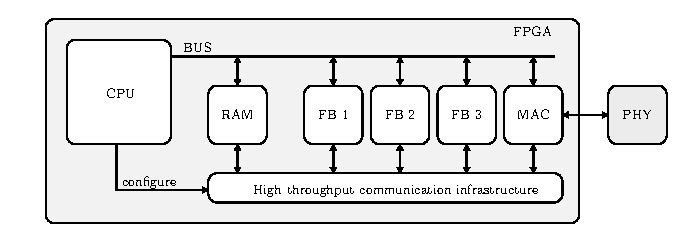
\includegraphics[width=\textwidth]{interconnectionInfrastructure.eps}
  \caption{The high throughput communication interface guarantees the functional blocks a worst case incoming and outgoing bandwith.}
  \label{interconnectionInfrastructure.eps}
  \end{center}
\end{figure}

\section{Organization of the Thesis}
The reminder of this thesis is organized in the following way: TODO!